\chapter{Setting up a breadboard}

\begin{figure}[!htb]
     \centering
     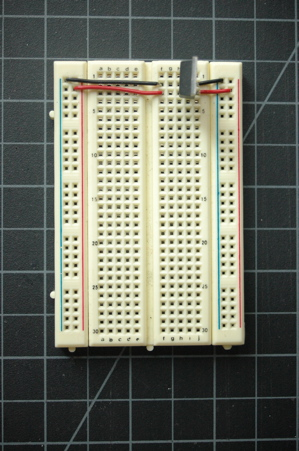
\includegraphics[scale=0.8]{img/breadboard/bboard_vreg_3.jpg}
     \caption{breadboard}
     \label{breadboard}
\end{figure}

Solderless beadboards are the quickest tools for prototyping a new circuit. For a detailed description of a breadboard, check these notes.

The picture at left shows a typical breadboard with a 7805 5-volt voltage regulator mounted on it. There are several rows of holes for components. The holes on the breadboard are separated by 0.1-inch spaces, and are organized in many short rows in the center, and in two long rows down each side of the board. The short horizontal rows in the middle are separated by a center divider. The pattern varies from model to model; some breadboards have only one strip down each side , others have multiple side rows, and some have no side rows.

On each side of the board are two long rows of holes, with a blue or a red line next to each row. All the holes in each of these lines are connected together with a strip of metal in the back. In the center are several short rows of holes separated by a central divider. All of the five holes in each row in the center are connected with a metal strip as well. This allows you to use the holes in any given row to connect components together. To see which holes are connected to which, take a multimeter and a couple of wires, set the multimeter to measure continuity, stick the two wires in two holes, and measure them with the multimeter. If the meter indicates continuity, then the two holes in question are connected.

\begin{figure}[!htb]
     \centering
     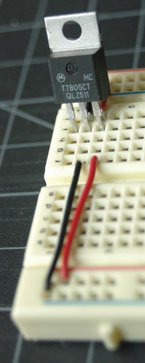
\includegraphics[scale=0.8]{img/breadboard/bboard_vreg_2.jpg}
     \caption{breadboard}
     \label{breadboard}
\end{figure}

The reason for the center divider is so that we can mount integrated circuit chips, like a microprocessor, on the breadboard. IC chips typically have two rows of pins that we need to connect other components to. The center row isolates the two rows from each other, and gives us several holes connected to each pin, so we can connect other components.

\textbf{When you start to put components on your breadboard, avoid adding, removing, or changing components on a breadboard whenever the board is powered. You risk shocking yourself and damaging your components.}

\begin{figure}[!htb]
     \centering
     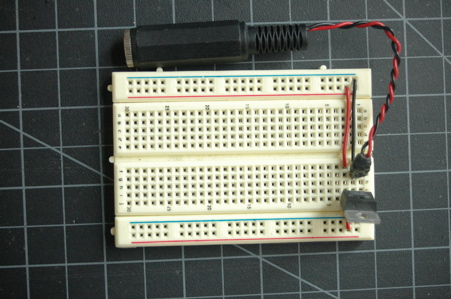
\includegraphics[scale=0.8]{img/breadboard/bboard_vreg_power_conn.jpg}
     \caption{breadboard}
     \label{breadboard}
\end{figure}

The regulator in the picture above is there to supply 5 volts to the two red side rows. The two blue side rows are connected to ground. These will be your power and ground bus rows. They give you lots of convenient places to connect to power or ground as needed. The red and black wires (red for power, black for ground) connect the bus rows to the rows where the regulator's ground and output pins are plugged in. The image at right shows a closeup on the connections to the regulator pins' rows.
With your board connected like this, you'll be able to build many different 5-volt circuits on the board. The last thing you need to add is a power connector to connect 8 - 12 volts DC to supply power for the voltage regulator. The image below shows a power connector connected to the input and ground pins of the voltage regulator.
